% =====================================================================
%  PG II — new section: "The Delta-x Structure and the Geometry of
%  Doubled Twins"
%
%  INSERTION: place immediately after \section{Empirical Verification}
%  (\label{sec:empirical}) and before the Twin-Ramanujan section.
%
%  PREAMBLE REQUIREMENTS (add to PG_II_AngleRecord.tex if absent):
%     \usepackage{graphicx}
%     \graphicspath{{../figures/}}     % figures live in Twin Bertrand/figures/
%
%  BIBLIOGRAPHY: add \bibitem{FS1} (Factor Skyline, Zenodo DOI
%  10.5281/zenodo.18275273) and \bibitem{MS2004} (Montgomery--Soundararajan).
%  Theorem 4.7a referenced below lives in FS1, sec. 4.3.1. The escape/template
%  framing in the Synthesis is attributed to FS1 (no separate bridge cite).
%
%  NOTATION (consistent with PG II): T_k = k-th twin lower-member;
%  G_k = T_{k+1}-T_k (twin gap, as in the twin-gap growth law of
%  Section~\ref{sec:empirical}). The local-density estimator is written
%  \widehat\lambda_k here (it is the rho_k of the companion Delta-x note,
%  renamed to avoid clash with the angle-record rho of Section~\ref{sec:angle}).
%
%  All numbers: uniform sieve to N = 10^8, 239,101 twin pairs / 239,100
%  gaps; reproduced by scripts/pg_deltax_unified.py.
% =====================================================================

\section{The \texorpdfstring{$\Delta x$}{Delta x} Structure and the Geometry of Doubled Twins}\label{sec:deltax}

The dyadic formulation of $(\mathrm{TPB})$ in Section~\ref{sec:tpb} and the
$2P$-beats lemma of Section~\ref{sec:2P} both turn on the map $T\mapsto 2T$.
This section studies that map directly as a geometric object: we place the
\emph{doubled} twins on a prime-rank axis and analyze the resulting gap
sequence. The picture is a near-perfect line whose slope obeys an explicit
$1/\log$ law, and whose microscopic fluctuations are inherited entirely from
the twin-gap distribution $G_k$ already studied in
Section~\ref{sec:empirical}.

\subsection{The doubled-twin shadow}\label{sec:deltax-def}

Let $T_k$ denote the $k$-th twin lower-member, so that
$\pi_2(x)=\#\{k:T_k\le x\}$. Place the primes on an evenly spaced
\emph{prime-rank} axis (the $i$-th prime at abscissa $i$) and drop each
doubled twin $2T_k$ onto it. Since $2T_k$ is even it falls strictly between
two consecutive primes, at abscissa $\pi(2T_k)$. Plotting
\[
   (x_k,y_k)=\bigl(\pi(2T_k),\,k\bigr)
\]
yields a strikingly linear point set (least-squares $R^2\approx 0.996$ over
the first hundred pairs). The governing object is the gap sequence

\begin{definition}\label{def:deltax}
For consecutive twins,
\[
   \Delta x_k \;=\; \pi(2T_{k+1})-\pi(2T_k)
   \;=\; \#\{\,q\text{ prime}: 2T_k<q\le 2T_{k+1}\,\},
\]
the number of primes in the doubled-twin window $(2T_k,2T_{k+1}]$.
\end{definition}

Because the ordinate increases by exactly $1$ from one twin to the next, the
local slope of the shadow between consecutive points is
\[
   \mathrm{slope}_k=\frac{y_{k+1}-y_k}{x_{k+1}-x_k}=\frac{1}{\Delta x_k}.
\tag{$\ast$}\label{eq:slope}
\]
From $\pi(2T)\sim 2T/\log T$ and $\pi_2(T)\sim 2C_2\,T/(\log T)^2$ the trend
relating the axes is $\pi(2T)\approx(\log T/C_2)\,\pi_2(T)$, a line of slope
$\approx C_2/\log T$; the entire shape of the shadow, line and fluctuation
alike, is encoded in $(\Delta x_k)$.

\subsection{Distribution of \texorpdfstring{$\Delta x$}{Delta x}}\label{sec:deltax-dist}

Over all $239\,101$ twin pairs with $2(T_k+2)\le 10^8$ ($239\,100$ gaps), the
sequence $\Delta x_k$ has mean $24.10$, median $17$, standard deviation
$23.02$, maximum $332$, with $3\,819$ zero values (consecutive doubled twins
sharing a prime slot). The distribution is unimodal with mode in $[10,20)$
and a long right tail (Figure~\ref{fig:deltax-hist}); the standard deviation
nearly equals the mean, the signature of a heavy-tailed, roughly exponential
spacing. Thus $\Delta x$ is highly irregular, not concentrated near any
preferred value.

\begin{figure}[h]
\centering
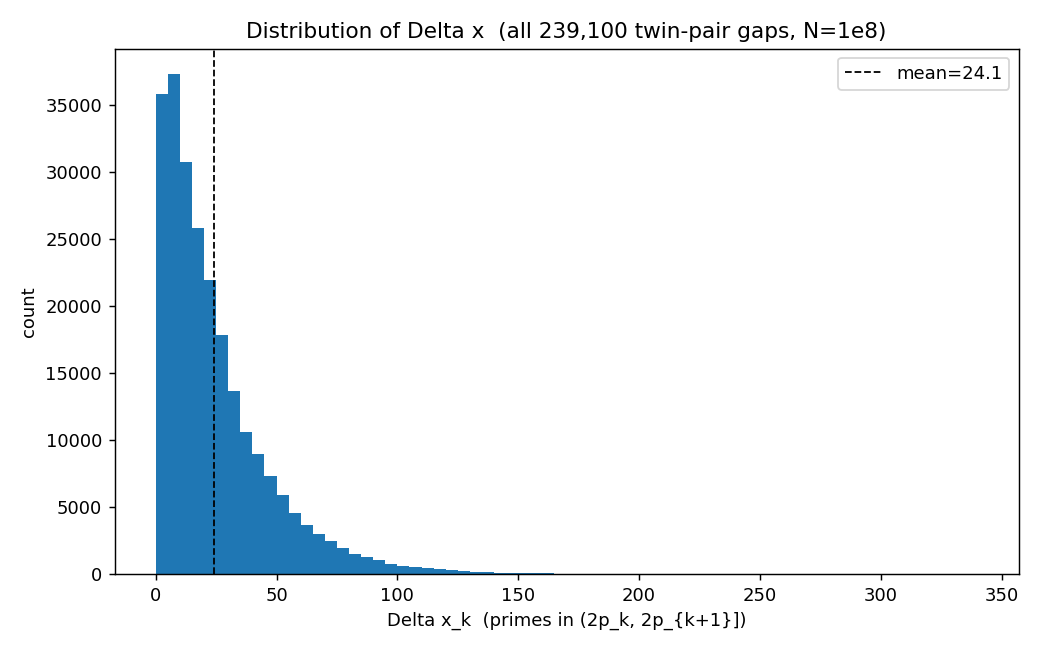
\includegraphics[width=0.8\textwidth]{deltax_histogram}
\caption{Distribution of $\Delta x_k$ over all $239\,100$ twin-pair gaps
(bins of width $5$; dashed line at the mean $24.1$). Mode in $[10,20)$, a
spike at $\Delta x=0$, and a thin right tail to $332$.}
\label{fig:deltax-hist}
\end{figure}

\subsection{The slope-drift law}\label{sec:deltax-slope}

By \eqref{eq:slope} the macro-slope of the shadow over a block of pairs is the
aggregate $1/\overline{\Delta x}$. (The per-step average
$\mathrm{mean}(1/\Delta x)$ is inadmissible: it is undefined on the $3\,819$
zero windows and Jensen-biased otherwise.) Differentiating the densities,
\[
   \mathrm{slope}
   =\frac{dk}{d\pi(2T)}
   =\frac{2C_2/(\log T)^2}{2/\log(2T)}
   =\frac{C_2\,\log(2T)}{(\log T)^2},
\tag{$\ast\ast$}\label{eq:slope-theory}
\]
whose leading coefficient is exactly $C_2=C_H/2$, half the Factor-Skyline
twin constant $C_H=2C_2$ established in Theorem~4.7a of the Factor Skyline
foundation paper~\cite{FS1}. Equation~\eqref{eq:slope-theory} exceeds the
crude $C_2/\log(2T)$ by the factor $(\log(2T)/\log T)^2\approx 1.1$.
Table~\ref{tab:deltax-slope} confirms~\eqref{eq:slope-theory} to $1$--$2\%$
across five decades.

\begin{table}[h]
\centering
\caption{Decade slope drift of the doubled-twin shadow. Empirical aggregate
slope $1/\overline{\Delta x}$ versus the refined prediction
$C_2\log(2T)/(\log T)^2$.}\label{tab:deltax-slope}
\begin{tabular}{lrrrr}
\toprule
decade of $T_k$ & $N$ & $\overline{\Delta x}$ & emp.\ slope & ratio to \eqref{eq:slope-theory} \\
\midrule
$[10^2,10^3)$        & $27$       & $9.70$  & $0.10305$ & $0.809$ \\
$[10^3,10^4)$        & $170$      & $11.50$ & $0.08696$ & $1.009$ \\
$[10^4,10^5)$        & $1\,019$   & $15.45$ & $0.06471$ & $0.982$ \\
$[10^5,10^6)$        & $6\,945$   & $18.85$ & $0.05304$ & $0.990$ \\
$[10^6,10^7)$        & $50\,811$  & $22.08$ & $0.04530$ & $1.004$ \\
$[10^7,5\cdot10^7)$  & $180\,120$ & $24.93$ & $0.04011$ & $0.998$ \\
\bottomrule
\end{tabular}
\end{table}

The slope drifts monotonically downward, $0.103\to0.040$, exactly the $1/\log$
behavior; the first decade $[10^2,10^3)$ is the sole outlier, in the
non-asymptotic regime. A free two-term fit
$\mathrm{slope}\approx A/L+B/L^2$ in $L=\log(2T)$ gives $A=0.795$, $B=-0.653$;
the apparent excess of $A$ over $C_2$ is an artifact of the bare
parametrization (expanding \eqref{eq:slope-theory} in $L$ gives
$A=C_2=0.660$, $B=2C_2\log2=0.915$), and the direct comparison of
Table~\ref{tab:deltax-slope} is the robust statement. Figure~\ref{fig:slope}
shows the decade points threading the backbone~\eqref{eq:slope-theory}.

\begin{figure}[h]
\centering
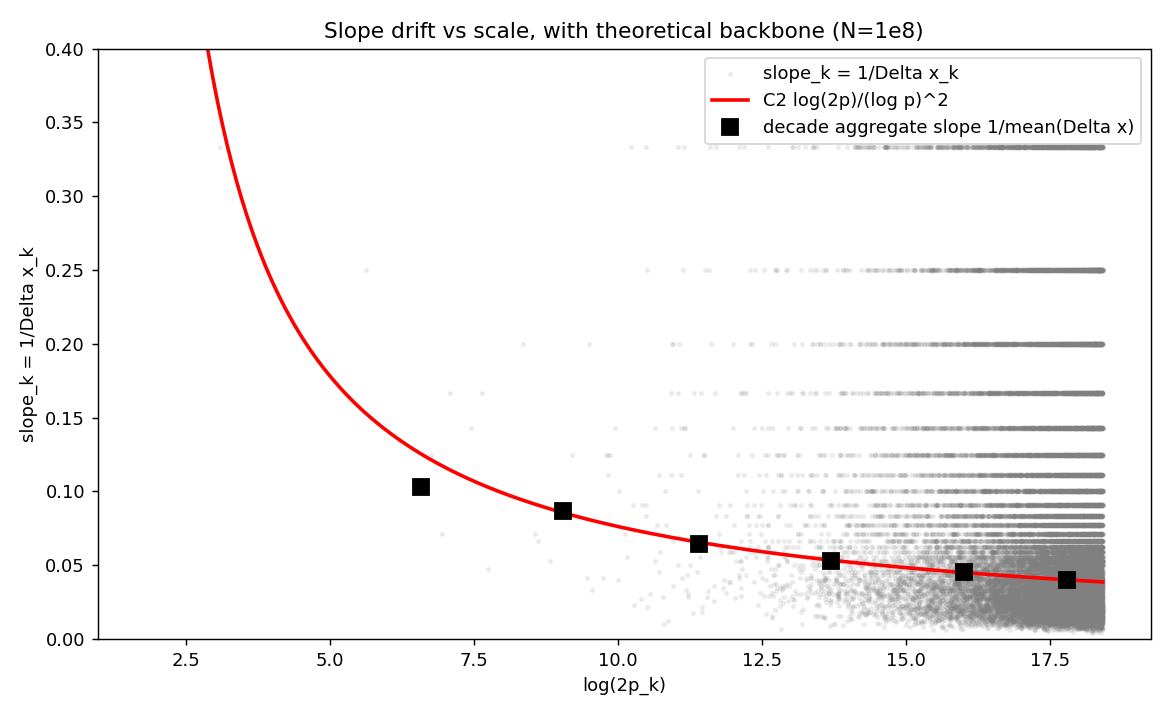
\includegraphics[width=0.85\textwidth]{slope_vs_log2p}
\caption{Local slope $1/\Delta x_k$ (gray, $30\,000$-point subsample) versus
$\log(2T_k)$, with the backbone $C_2\log(2T)/(\log T)^2$ (red) and the six
decade-aggregate slopes (squares). The discrete stripes are the admissible
values $1,\tfrac12,\tfrac13,\dots$ of $1/\Delta x$.}
\label{fig:slope}
\end{figure}

\subsection{Variance decomposition: the twin gap dominates}\label{sec:deltax-var}

Write the window length as $2G_k$, where $G_k=T_{k+1}-T_k$ is the twin gap of
Section~\ref{sec:empirical}, and define the local-density estimator
$\widehat\lambda_k=\Delta x_k/(2G_k)$, so that
\[
   \Delta x_k = 2G_k\cdot\widehat\lambda_k,\qquad
   \log\Delta x_k=\log(2G_k)+\log\widehat\lambda_k.
\]
The estimator $\widehat\lambda_k$ tracks the prime number theorem value
$\lambda_k=1/\log(2T_k)$ closely: the ratio
$r_k=\widehat\lambda_k/\lambda_k$ has mean $0.992$, median $0.995$, and
standard deviation $0.285$ (Figure~\ref{fig:scatter}). Partitioning the
log-variance,
\[
   \mathrm{Var}(\log\Delta x)=1.122,\quad
   \mathrm{Var}(\log 2G)=1.142,\quad
   \mathrm{Var}(\log\widehat\lambda)=0.076,
\]
the width term alone accounts for essentially the entire variance (the
density term is cancelled by a negative covariance). Equivalently, the
coefficients of variation are $0.955$ for $\Delta x$ and $0.953$ for $G$, but
only $0.300$ for $\widehat\lambda$.

\begin{proposition}\label{prop:deltax-var}
The fluctuations of $\Delta x_k$ are inherited essentially entirely from the
twin-gap sequence $G_k$, not from the local prime density: the
density factor $\widehat\lambda_k$ is rigid (it hugs $1/\log(2T)$ with
$\pm 29\%$ scatter), whereas $G_k$ is heavy-tailed (range $2$ to $2\,832$,
coefficient of variation $0.95$).
\end{proposition}

In particular the slope identity~\eqref{eq:slope} factors as
$\mathrm{slope}_k\approx\log(2T_k)/(2G_k)$: the slowly growing
$\log(2T_k)$ is the deterministic drift of Table~\ref{tab:deltax-slope},
while $1/G_k$ is the noise. The twin-gap growth law of
Section~\ref{sec:empirical} therefore governs the scatter of the doubled-twin
shadow directly.

\begin{figure}[h]
\centering
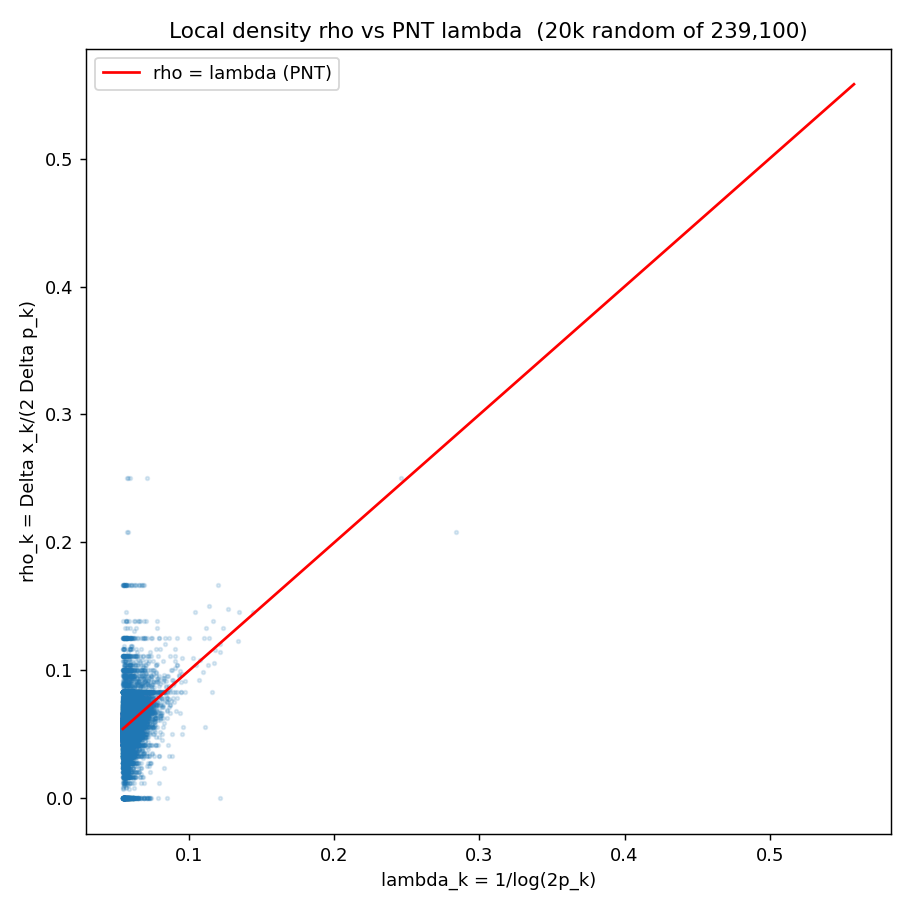
\includegraphics[width=0.7\textwidth]{lambda_rho_scatter}
\caption{Local density $\widehat\lambda_k=\Delta x_k/(2G_k)$ versus the PNT
prediction $\lambda_k=1/\log(2T_k)$ ($20\,000$-point subsample), with the
diagonal $\widehat\lambda=\lambda$. The cloud is centered on the diagonal
(mean ratio $0.99$) with bounded $\pm 29\%$ spread.}
\label{fig:scatter}
\end{figure}

\subsection{A Poisson-mixture model and the chance nature of collinearity}\label{sec:deltax-poisson}

The linearity of the shadow invites the question whether three or more
consecutive points are ever exactly collinear. By~\eqref{eq:slope} this asks
whether $\Delta x_k=\Delta x_{k+1}$. Empirically, equal adjacent gaps occur in
only $1.95\%$ of positions; the longest exact straight run in $239\,100$ gaps
is six points, occurring once. So collinearity beyond pairs is rare and
unstructured.

This rate is precisely what chance predicts. Modeling the primes near $2T_k$
as an inhomogeneous Poisson process of intensity $1/\log t$, the count
$\Delta x_k$ is Poisson with mean
$\mu_k\approx 2G_k/\log(2T_k)$; since $G_k$ varies widely, the marginal of
$\Delta x$ is a \emph{Poisson mixture}, strongly overdispersed (variance
$529.8$ against mean $24.10$, ratio $\approx 22$). For independent draws from
the empirical marginal, the expected coincidence rate is
$\sum_v\Pr[\Delta x=v]^2=1.99\%$, matching the observed $1.95\%$; a single
Poisson of the same mean would predict $5.76\%$, far too high because it is
too concentrated. Hence the collinearity rate carries no signal: it is the
chance coincidence rate of an overdispersed, twin-gap-driven gap process. (This
overdispersion is the gap-count companion of the extreme-gap overshoot
documented in Section~\ref{sec:empirical}.)

\subsection{Scale-collapse of the conditional gap}\label{sec:deltax-collapse}

Normalizing by the full conditional mean, set $Z_k=\Delta x_k/\mu_k$ with
$\mu_k=2G_k/\log(2T_k)$; algebraically $Z_k=r_k$ of
Section~\ref{sec:deltax-var}. Binning by decades of $T_k$, the distribution of
$Z_k$ collapses onto a single scale-invariant shape: it is unimodal, centered
just below $1$, with standard deviation $\approx 0.28$ at every scale, and the
Kolmogorov--Smirnov distance between decades falls to $0.021$ between the two
largest (Table~\ref{tab:deltax-collapse}).

\begin{table}[h]
\centering
\caption{Scale-collapse of $Z_k=\Delta x_k/\mu_k$. The KS column is the
distance to the next decade.}\label{tab:deltax-collapse}
\begin{tabular}{lrrrr}
\toprule
decade of $T_k$ & $N$ & $\overline{Z}$ & $\mathrm{std}\,Z$ & KS to next \\
\midrule
$[10^2,10^3)$        & $27$       & $0.940$ & $0.256$ & $0.166$ \\
$[10^3,10^4)$        & $170$      & $0.956$ & $0.277$ & $0.071$ \\
$[10^4,10^5)$        & $1\,019$   & $0.976$ & $0.256$ & $0.063$ \\
$[10^5,10^6)$        & $6\,945$   & $0.991$ & $0.290$ & $0.026$ \\
$[10^6,10^7)$        & $50\,811$  & $0.992$ & $0.288$ & $0.021$ \\
$[10^7,5\cdot10^7)$  & $180\,120$ & $0.993$ & $0.284$ & --- \\
\bottomrule
\end{tabular}
\end{table}

The normalization removes the twin-gap-driven overdispersion entirely: the
coefficient of variation falls from $0.955$ for $\Delta x$ to $0.287$ for $Z$,
and is scale-stable. What remains is \emph{not} pure Poisson shot noise: a
Poisson model predicts $\mathrm{std}\,Z\approx1/\sqrt{\overline{\Delta x}}$,
which would fall through $0.32,0.30,0.25,0.23,0.21,0.20$ across the six
decades, whereas the observed spread holds near $0.28$ and increasingly
exceeds the Poisson reference. The conditional gap is thus mildly
super-Poissonian, consistent with the excess variance of primes in short
intervals~\cite{MS2004}, and the residual is a genuine, scale-free arithmetic
fluctuation.

\subsection{Synthesis}\label{sec:deltax-synth}

The doubled-twin shadow decomposes cleanly: a deterministic $1/\log$ slope
drift (Table~\ref{tab:deltax-slope}, leading constant $C_2=C_H/2$) carrying
twin-gap-driven, scale-free counting noise
(Proposition~\ref{prop:deltax-var}, Section~\ref{sec:deltax-collapse}). The
three successive normalizations form a ladder of decreasing variability,
$\Delta x\ (\mathrm{CV}=0.955)\to\widehat\lambda\ (0.300)\to Z\ (0.287)$, each
peeling away one structural layer (window width, then density trend) until
only the irreducible arithmetic fluctuation remains.

In the Factor-Skyline reading that motivates $(\mathrm{TPB})$ (the
coverage/escape architecture of~\cite{FS1}), this is exactly the split between
what the coverage template supplies for free and what the escape layer cannot:
the
candidate windows and their density --- the deterministic backbone above ---
are template structure, governed by the same constant $C_H$ that
Theorem~4.7a~\cite{FS1} identifies with the Hardy--Littlewood singular series,
while the scale-free residual $Z$ is the escape randomness. The geometry of
doubled twins thus renders the $(\mathrm{TPB})$ density mechanism visible: a
predictable trend that guarantees candidates, dressed in a fluctuation that no
coverage argument controls.
